% =====================================================================
%  Chapter 7 -- Stage 4: a change of state decided by speed (R_i sweep)
% =====================================================================
\chapter{Stage 4: A Change of State Decided by Speed}\label{ch:stage4}
\chapterlists

We now sweep the input resistor, so that the gain follows one fixed path in every run, and ask
Criterion~3: \emph{does the long-time state depend on the speed alone?}

\section{What we did}\label{sec:s4-setup}

Configuration B (\cref{fig:two-configs}b, \cref{tab:configs}): $\RF=\SI{90}{\kilo\ohm}$ fixed, $\Ri$
sweeping \SIrange{41}{51}{\kilo\ohm} along the staircase of \cref{fig:staircase}, so $G$ moves between
3.20 and 2.76, about twice as much per step as in configuration A. Two further differences:
\begin{itemize}
  \item \textbf{Every run starts oscillating.} Before the sweep the wiper rests where $G$ is highest, so
        the first downward pass switches the oscillation \emph{off}. The question is whether it returns.
  \item \textbf{Most of the path lies below threshold.} With the measured bench threshold only seven of 32
        positions have $G>\Gc$, so $\Gp<\Gm$: regime~(c) of \cref{sec:budget}.
\end{itemize}
Nineteen runs were recorded with $\tau=\SIrange{37}{100}{\milli\second}$
($\lambda=\SIrange{3.2}{8.7}{\kilo\ohm\per\second}$), each at least a minute long with 12 to 28 cycles.

\section{Same path, two fates}\label{sec:s4-twofates}

\begin{figure}[!htb]
  \centering
  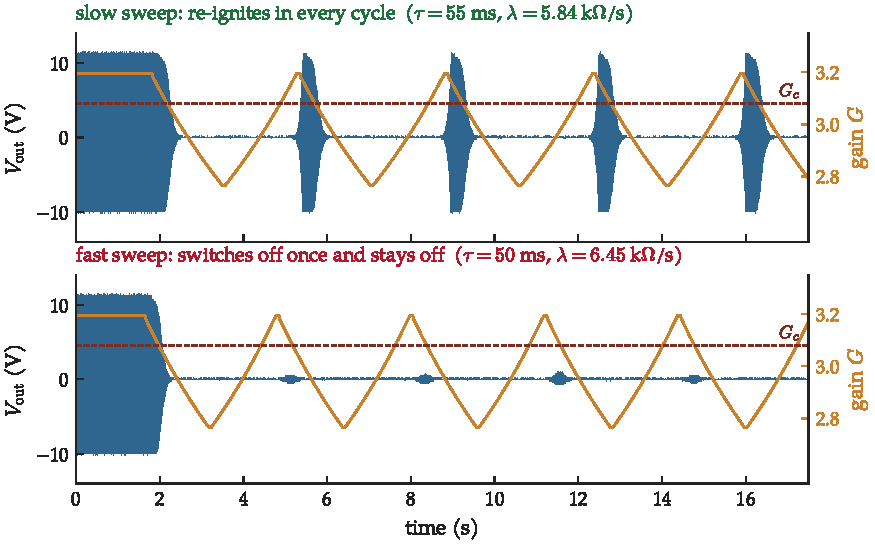
\includegraphics[width=0.9\linewidth]{fig_s4_twofates}
  \caption[Stage 4: same path, two fates]{The same gain path (orange) at two speeds; dashed: threshold.
  Top, $\tau=\SI{55}{\milli\second}$: the oscillation is reborn each time the gain rises above threshold.
  Bottom, $\tau=\SI{50}{\milli\second}$: it switches off once and never returns.}
  \label{fig:s4-twofates}
\end{figure}

In \cref{fig:s4-twofates} the gain follows exactly the same path in both runs, crossing the threshold
the same number of times; the step times differ by $10\%$. At $\tau=\SI{55}{\milli\second}$ every rise
above threshold restores full size, for the whole record. At $\tau=\SI{50}{\milli\second}$ the
oscillation dies on the first downward pass and never returns; each later rise produces only a swelling
of a few per cent, lost again on the next pass. Same circuit, path and noise: the speed alone decides the
state.

\section{All the runs}\label{sec:s4-all}

The 19 runs split into two groups with no overlap (\cref{fig:s4-gallery,tab:s4-runs}). For
$\tau\ge\SI{53}{\milli\second}$ (ten runs) the oscillation re-ignites every cycle; all but two reach full
size in every cycle, and those two miss only once in fifteen or sixteen. For $\tau\le\SI{52}{\milli\second}$
(nine runs) it switches off once and stays off: none of its 187 cycles rises above half of full size.

\begin{figure}[!htbp]
  \centering
  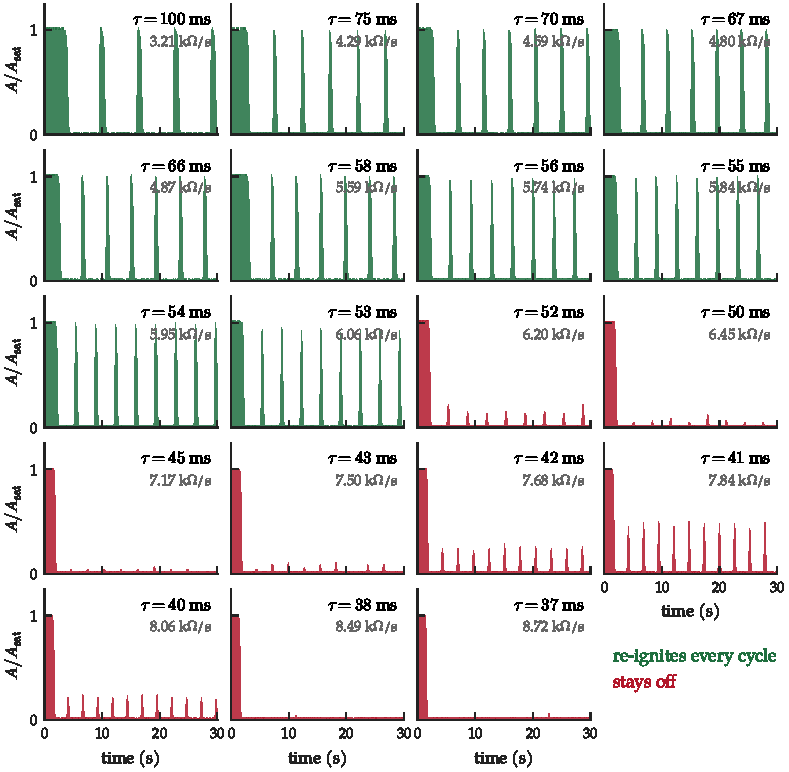
\includegraphics[width=0.72\linewidth]{fig_s4_gallery}
  \caption[Stage 4: every run]{Envelope of every run (first \SI{30}{\second}), slow (top left) to fast
  (bottom right). Green: re-ignites every cycle. Red: off for good.}
  \label{fig:s4-gallery}
\end{figure}

\begin{table}[!htb]
  \centering
  \small
  \renewcommand{\arraystretch}{1.05}
  \begin{tabular}{@{}rrcccl@{}}
    \toprule
    $\tau$ (ms) & $\lambda$ (\si{\kilo\ohm\per\second}) & cycles & re-ignited & peak range ($A/\Asat$) & long-time state \\
    \midrule
    100 & 3.21 & 21 & 21 & 1.00\,--\,1.02 & \textcolor{upcol}{re-ignites} \\
     75 & 4.29 & 28 & 28 & 0.96\,--\,1.02 & \textcolor{upcol}{re-ignites} \\
     70 & 4.59 & 12 & 12 & 1.00\,--\,1.02 & \textcolor{upcol}{re-ignites} \\
     67 & 4.80 & 13 & 13 & 1.00\,--\,1.01 & \textcolor{upcol}{re-ignites} \\
     66 & 4.87 & 13 & 13 & 1.00\,--\,1.02 & \textcolor{upcol}{re-ignites} \\
     58 & 5.59 & 15 & 14 & 0.56\,--\,1.02 & \textcolor{upcol}{re-ignites} \\
     56 & 5.74 & 15 & 15 & 0.96\,--\,0.99 & \textcolor{upcol}{re-ignites} \\
     55 & 5.84 & 16 & 16 & 0.99\,--\,1.01 & \textcolor{upcol}{re-ignites} \\
     54 & 5.95 & 16 & 16 & 0.99\,--\,1.01 & \textcolor{upcol}{re-ignites} \\
     53 & 6.06 & 16 & 15 & 0.71\,--\,0.96 & \textcolor{upcol}{re-ignites} \\
    \midrule
     52 & 6.20 & 17 & 0 & 0.04\,--\,0.29 & \textcolor{dncol}{stays off} \\
     50 & 6.45 & 17 & 0 & 0.02\,--\,0.18 & \textcolor{dncol}{stays off} \\
     45 & 7.17 & 20 & 0 & 0.02\,--\,0.07 & \textcolor{dncol}{stays off} \\
     43 & 7.50 & 21 & 0 & 0.02\,--\,0.11 & \textcolor{dncol}{stays off} \\
     42 & 7.68 & 21 & 0 & 0.20\,--\,0.28 & \textcolor{dncol}{stays off} \\
     41 & 7.84 & 21 & 0 & 0.43\,--\,0.50 & \textcolor{dncol}{stays off} \\
     40 & 8.06 & 22 & 0 & 0.18\,--\,0.24 & \textcolor{dncol}{stays off} \\
     38 & 8.49 & 24 & 0 & 0.02\,--\,0.04 & \textcolor{dncol}{stays off} \\
     37 & 8.72 & 24 & 0 & 0.02\,--\,0.07 & \textcolor{dncol}{stays off} \\
    \bottomrule
  \end{tabular}
  \caption[Stage 4: summary of all runs]{All runs. ``Re-ignited'': cycles reaching at least 90\% of full
  size; peak range: smallest and largest cycle peak.}
  \label{tab:s4-runs}
\end{table}

Among the runs that stay off, the peak per cycle does not fall steadily with rate, as $\Gp\propto1/\lambda$
would suggest: it is largest, 0.43--0.50, at $\tau=\SI{41}{\milli\second}\approx3T_{0}$ (\cref{tab:s4-runs}).
A possible cause, outside the envelope theory, is phase locking: when a step lasts a whole number of
periods, the transient of every wiper move arrives at the same phase. No run crosses $\lamc$ because of it.

\subsection{Cycle map and tipping diagram}

The cycle map (\cref{fig:s4-cyclemap}a) shows the peak of every cycle of every run. Bright rows reach full
size from first cycle to last; dark rows never recover, even 24 cycles later. These are long-time states,
not transients, separated sharply between \num{53} and \SI{52}{\milli\second} per step.

\begin{figure}[!htb]
  \centering
  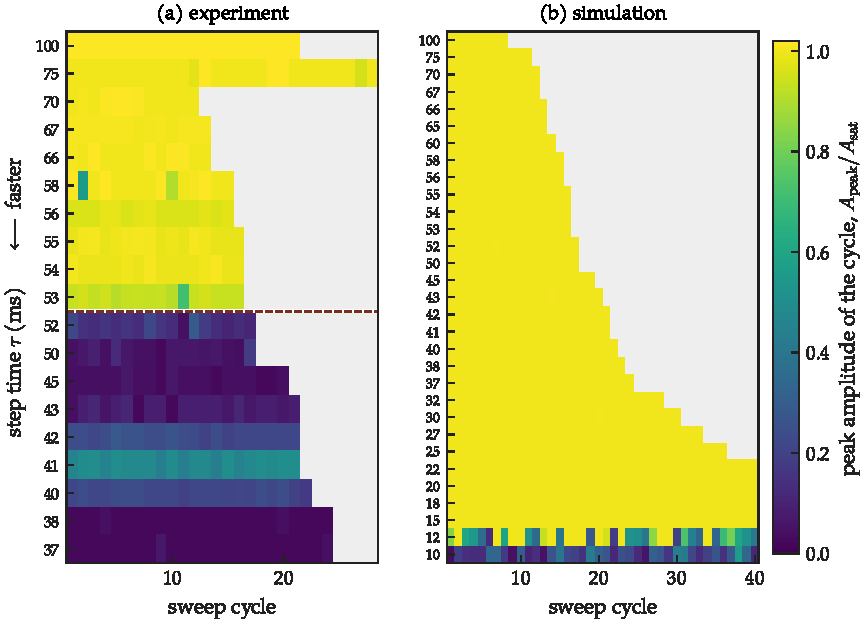
\includegraphics[width=0.75\linewidth]{fig_s4_cyclemap}
  \caption[Stage 4: cycle maps]{Cycle maps: peak amplitude of every cycle, sweeps getting faster from top
  to bottom. (a)~Experiment; dashed: boundary between the two states. (b)~Simulation, down to
  $\tau=\SI{10}{\milli\second}$. Grey: beyond the record.}
  \label{fig:s4-cyclemap}
\end{figure}

The tipping diagram (\cref{fig:s4-tipping}) plots every cycle peak against the rate of its run. Below a
critical rate every point is at full size, above it every point lies far below, with
\begin{equation}
  \boxed{\;\SI{6.06}{\kilo\ohm\per\second} < \lamc < \SI{6.20}{\kilo\ohm\per\second}\;}
  \qquad (\SI{53}{\milli\second} > \tau_{c} > \SI{52}{\milli\second}) ,
  \label{eq:s4-lamc}
\end{equation}
a window of $2\%$ in rate.

\begin{figure}[!htb]
  \centering
  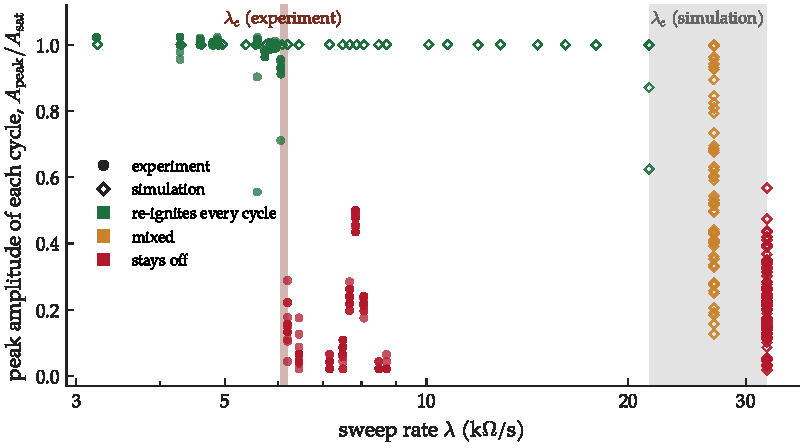
\includegraphics[width=0.75\linewidth]{fig_s4_tipping}
  \caption[Stage 4: the tipping diagram]{Tipping diagram: peak of every cycle against rate, experiment
  (filled) and simulation (open). Shaded bands: critical rates.}
  \label{fig:s4-tipping}
\end{figure}

\begin{keybox}
\textbf{Criterion 3 is met.} Along one fixed gain path, the long-time state is decided by the rate alone:
oscillating every cycle below $\lamc\approx\SI{6.1}{\kilo\ohm\per\second}$, quiet for good above it.
\end{keybox}

\section{Why the state changes}\label{sec:s4-why}

This is the growth budget of \cref{sec:budget}, sketched in \cref{fig:budget}. Each pass above threshold
allows growth by at most $e^{\Gp}$, which shrinks as $1/\lambda$ (\cref{eq:budget-rate}). If it suffices
to lift the oscillation from noise to full size, every cycle re-ignites; if not, the little growth
collected is lost on the longer stretch below threshold ($\Gm>\Gp$), and the circuit never climbs back.

With the measured threshold $\Gc=3.081$ (\cref{sec:s4-switchoff}), \cref{eq:Gp} gives at the experimental
critical rate
\begin{equation}
  \Gp(\lamc) = \frac{\wo\,\Delta R}{\lamc}\sum_{k}\bigl(G_{k}-\Gc\bigr)_{+} \approx 10.7\text{--}11.0 .
  \label{eq:s4-gamma}
\end{equation}
By \cref{eq:tip-condition} this equals $\ln(\Asat/\delta)$; with $\Asat=\SI{11.25}{\volt}$ it implies a
noise floor $\delta\approx\SI{0.2}{\milli\volt}$ (\cref{fig:s4-budget}). Because $\Gp$ depends steeply on
$\Gc$, the uncertainty $\pm0.003$ of $\Gc$ (\cref{sec:s4-switchoff}) makes this uncertain by a factor of
about 1.6: $\delta=0.2^{+0.13}_{-0.08}\,\si{\milli\volt}$. This is an order of magnitude below the effective
floor inferred from the Stage~2 switch-on coefficient in the same circuit, \SI{2.6}{\milli\volt}
(\cref{sec:s2-results}). Part of the difference may come from the rate-dependent effective floor at
switch-on (\cref{sec:s1-results}). The growth budget therefore explains the dependence of the critical rate
on rate and threshold quantitatively, but fixes the noise floor only to within an order of magnitude.

\begin{figure}[!htb]
  \centering
  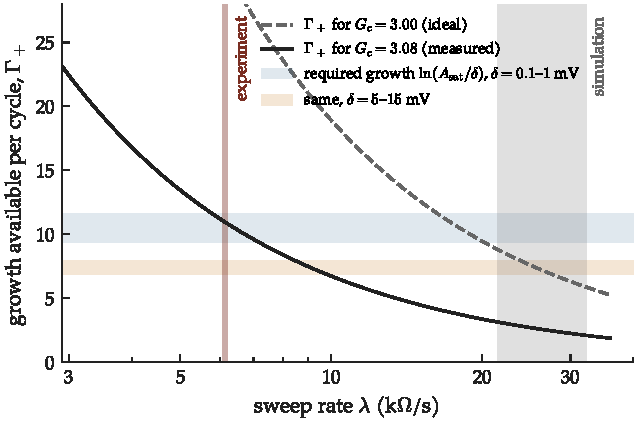
\includegraphics[width=0.55\linewidth]{fig_s4_budget}
  \caption[Stage 4: growth available per cycle]{$\Gp$ (\cref{eq:budget-rate}) against rate for the measured
  bench threshold (solid) and the ideal threshold (dashed). Horizontal bands: growth needed to climb from
  the noise floor. Vertical bands: observed critical rates.}
  \label{fig:s4-budget}
\end{figure}

\begin{whybox}[Why the critical rate is so sharp]
Only seven positions lie above threshold, each contributing in proportion to its distance from
$\Gc$. A shift of $\Gc$ by $0.01$ changes $\Gp$ by about 1.7, a factor of five to six in peak amplitude.
Near $\lamc$ the budget sits on a knife edge, and $2\%$ in rate tips it.
\end{whybox}

\section{The switch-off still follows \texorpdfstring{$\sqrt{\lambda}$}{the square root}}
\label{sec:s4-switchoff}

The first switch-off of each run is a single crossing of the kind treated in \cref{sec:ri-sweep}.
\Cref{fig:s4-switchoff} shows $\Ri$ at the 10\% point for the 18 runs whose trigger reference fixes it
reliably. The leading-order law gives
\begin{equation}
  R_{i,\mathrm{off}} = (\num{43.25 \pm 0.06})\,\si{\kilo\ohm} + (\num{14.9 \pm 0.7})\sqrt{\lambda} ,
  \label{eq:s4-off}
\end{equation}
slightly better than a fixed delay (rms \SI{28}{\ohm} against \SI{30}{\ohm}, AIC lower by 2.6). The exact law
\cref{eq:Ri-exact} gives the same intercept and is indistinguishable here, so the correction term of
\cref{eq:Ri-off} is negligible. At these rates the lag is only three to four potentiometer steps, so the
continuous-ramp derivation of \cref{sec:ri-sweep} is used at the edge of its validity.

\begin{figure}[!htb]
  \centering
  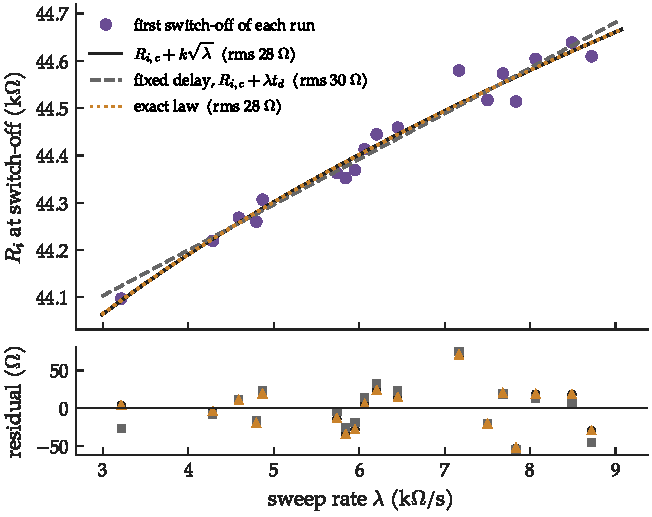
\includegraphics[width=0.6\linewidth]{fig_s4_switchoff}
  \caption[Stage 4: the switch-off point]{$\Ri$ at the first switch-off against rate, with the
  $\sqrt{\lambda}$ law (solid), a fixed delay (dashed) and the exact law \cref{eq:Ri-exact} (dotted).
  Bottom: residuals.}
  \label{fig:s4-switchoff}
\end{figure}

\paragraph{Threshold} The intercept gives
\begin{equation}
  \Gc = 1 + \frac{\RF}{R_{i,c}} = 1 + \frac{\SI{90}{\kilo\ohm}}{\SI{43.25}{\kilo\ohm}} = 3.081 \pm 0.003 ,
  \label{eq:s4-Gc}
\end{equation}
close to configuration A (3.07, \cref{eq:s2-Gc}). The difference, $0.3\%$, is within component
tolerances, since the two configurations use different fixed resistors. This is the $\Gc$ used in
\cref{sec:s4-why}.

\paragraph{Size of the lag} With $\Loff$ free, the exact law gives $\Loff=\num{1.18 \pm 0.11}$, about half of
$\ln 10$; equivalently the fitted coefficient is about three quarters of the predicted
$k_{i}=\SI{20.4}{\ohm^{1/2}\,\second^{1/2}}$. The law is the square root; its coefficient in this
configuration is smaller than the simple theory gives.

\section{The simulation shows the same tipping}\label{sec:s4-sim}

The protocol was simulated at 31 step times: the 19 experimental ones and twelve more down to
\SI{10}{\milli\second} (\cref{fig:s4-cyclemap}b, \cref{fig:s4-tipping}). From \num{100} down to
\SI{15}{\milli\second} the oscillation re-ignites every cycle (all but two of 61 at
\SI{15}{\milli\second}); at \SI{10}{\milli\second} it switches off and stays off. At \SI{12}{\milli\second}
the run is \emph{mixed}: 31 of 77 cycles ($40\%$) re-ignite, in no regular order, consistent with a
threshold at which the budget barely suffices and noise decides each cycle. The simulated
critical rate lies in
\begin{equation}
  \SI{21.5}{\kilo\ohm\per\second} < \lamc^{\text{sim}} < \SI{32.3}{\kilo\ohm\per\second} .
  \label{eq:s4-lamc-sim}
\end{equation}
The simulated circuit withstands faster sweeps for two reasons. With $\Gc$ exactly 3, thirteen positions
lie above threshold instead of seven (\cref{tab:budget-theory,fig:s4-budget}); and its effective noise
floor is larger ($\Lon=6.7$ in Stage~3, so $\delta\approx\SI{15}{\milli\volt}$), so less growth is needed.
With these values \cref{eq:lamc} gives $\lamc=\wo\,\Delta R\,S_{+}/\ln(\SI{13.9}{\volt}/\SI{15}{\milli\volt})
\approx\SI{27.6}{\kilo\ohm\per\second}$, inside the bracket of \cref{eq:s4-lamc-sim} and close to the mixed
run at \SI{26.9}{\kilo\ohm\per\second}. The nature of the transition is the same.

\section{A control: one sweep is not enough}\label{sec:s4-control}

Would a single fast pass also leave the circuit in a different final state? We simulated one sweep of
$\Ri$ across its full range, without return, along the smooth step of \cref{sec:simulation}, at 13 speeds
from \num{0.5} to \SI{100}{\kilo\ohm\per\second} (\cref{fig:s4-single}).

\begin{figure}[!htb]
  \centering
  \begin{subfigure}{\linewidth}
    \centering
    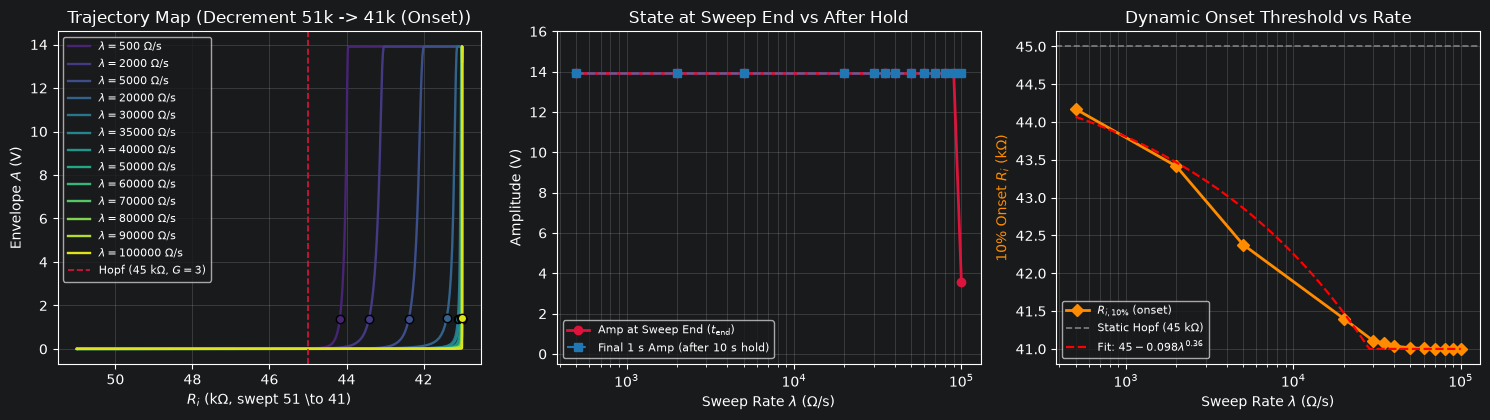
\includegraphics[width=0.8\linewidth]{deck_single_dec}
    \caption{Gain rising: $\Ri$ swept from \num{51} to \SI{41}{\kilo\ohm}}
  \end{subfigure}\\[4pt]
  \begin{subfigure}{\linewidth}
    \centering
    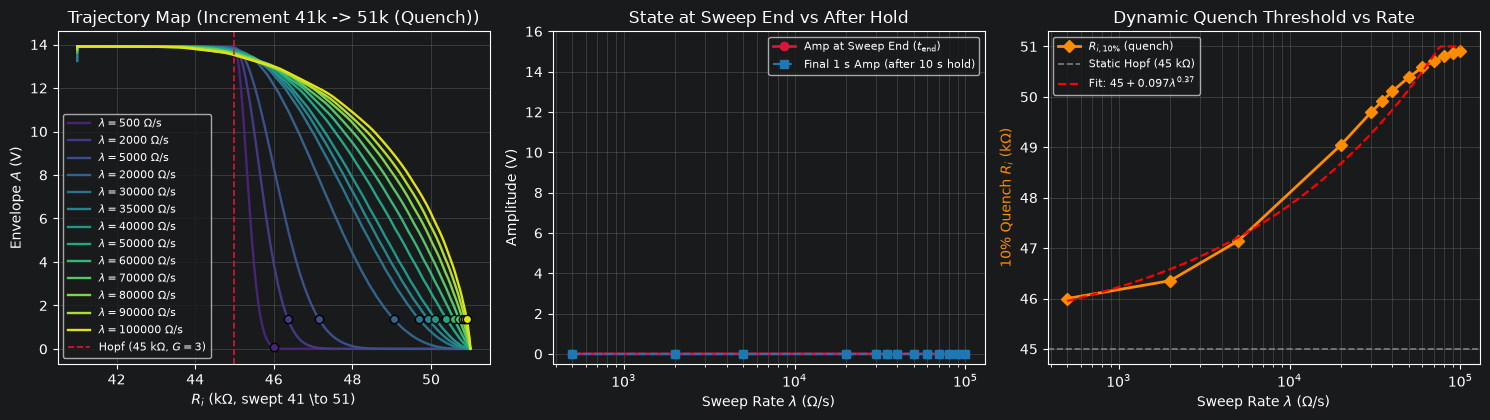
\includegraphics[width=0.8\linewidth]{deck_single_inc}
    \caption{Gain falling: $\Ri$ swept from \num{41} to \SI{51}{\kilo\ohm}}
  \end{subfigure}
  \caption[Stage 4: a single sweep (simulation)]{A single sweep (simulation). In each row: envelope
  against $\Ri$ for all rates (left), amplitude at the end of the sweep and after a hold (centre), and the
  switching point against rate (right). Every rising sweep ends oscillating at full size and every falling
  sweep ends quiet, at all rates; only the switching point moves.}
  \label{fig:s4-single}
\end{figure}

Raising the gain always ends at full size (\SI{13.9}{\volt}), at the fastest rates only during the hold
that follows the sweep; lowering it always ends quiet. The speed only shifts \emph{where} the switch
happens. The switch-off points, \num{45.67}, \num{46.33}, \num{47.09} and \SI{48.96}{\kilo\ohm} at
\num{0.5}, \num{2}, \num{5} and \SI{20}{\kilo\ohm\per\second}, agree to within \SI{50}{\ohm} with
\cref{eq:envelope} integrated along the actual path, which predicts \num{45.67}, \num{46.35}, \num{47.13}
and \SI{49.00}{\kilo\ohm} with no free parameter. Because the rate at threshold is $1.92\lambda$, these
points grow as $\sqrt{\lambda}$ with a coefficient $\sqrt{1.92}$ times the $k_{i}$ of \cref{eq:Ri-off}. One crossing produces a lag but never a
different final state; the tipping of this stage requires \emph{repeated} passes, each too short to
rebuild the oscillation from noise. It is a signature of rate-induced tipping under periodic driving.


\section{What this stage taught us}\label{sec:s4-learned}

\begin{learned}
\begin{itemize}[leftmargin=1.2em]
  \item \textbf{Same path, different fates}: below $\lamc$ every cycle re-ignites, above it the circuit
        stays quiet for good (Criterion~3).
  \item \textbf{Sharp critical rate}: $\SI{6.06}{\kilo\ohm\per\second}<\lamc<\SI{6.20}{\kilo\ohm\per\second}$,
        with no overlap among 19 runs.
  \item \textbf{Explained by the growth budget}: with $\Gc=3.081$, $\Gp\approx 11$ at $\lamc$.
  \item \textbf{Reproduced in simulation}, with a mixed run at its critical rate; a single sweep never tips.
\end{itemize}
\end{learned}
